\section{РАЗРАБОТКА СТРУКТУРНОЙ СХЕМЫ}


  \textbf{\subsection{Анализ технического задания}}
  \vspace{1em}
  Выбор структурной схемы усилителя определяется рядом параметров и условиями эксплуатации. Количество каскадов определяется величиной входного и выходного сигналов, выбор источника питания, радиоэлементов и основ построения схемы производится с учетом предназначения устройства, требований к сложности, условий эксплуатации.\par
  Исходные данные: \par 
  \begin{itemize}
  \item $P_{\text{н}} = 8$ (Вт) ~--~ номинальная выходная мощность 
  \item $R_{\text{н}} = 2$ (Ом) ~--~ сопротивление нагрузки 
  \item $E_{\text{г}} = 45$ (мВ) ~--~ ЭДС источника сигнала 
  \item $R_{\text{г}} = 10$ (кОм) ~--~ внутреннее сопротивление источника сигнала 
  \item $K_{\text{г}} = 1$ (\%) ~--~ допустимый коэффициент гармоник 
  \item $f_{\text{н}} = 10$ (Гц) ~--~ нижняя предельная частота  
  \item $f_{\text{в}} = 18$ (кГц) ~--~ верхняя предельная частота  
  \item $M = 3$ (дБ) ~--~ неравномерность АЧХ в полосе  
  \item $\Delta b_{\text{т}} = \pm 14$ (дБ) ~--~ пределы регулировки тембра  
  \item $T^{o}_{\text{мах}} = 40$ ($^oC$) ~--~ максимальное значение температуры окружающей среды  
  \item Регулировка громкости ~--~ плавная
  \item Вид аппаратуры ~--~ автомобильная
  \item Группа сложности ~--~ 0
  \end{itemize}
 
  Структурная схема усилителя сигналов звуковой частоты: \par
  \begin{figure}[htbp]
    \center{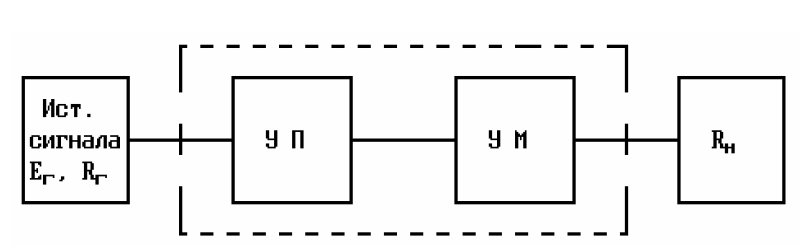
\includegraphics[width=0.8\linewidth]{picture_1}}
    \caption{Упрощенная структурная схема усилителя}
    \label{figure:p1_1}
  \end{figure}
  
  Предварительный усилитель (УП) осуществляет усиление сигнала по напряжению до уровня, необходимого для работы усилителя мощности (УМ). Кроме того, в УП осуществляются оперативные регулировки уровня сигнала (громкости) и тембра (коррекция АЧХ). \par 
Усилитель мощности обеспечивает основное усиление мощности до уровня, заданного в ТЗ. 


